
\documentclass{article}

\usepackage[french]{babel}
\usepackage[T1]{fontenc}
\usepackage[utf8]{inputenc}
\usepackage{graphicx}
\usepackage{eurosym}
\usepackage {times}
\usepackage{fancyhdr}
\usepackage{bm}


\title{Projet DotNet par KMnO4\\~Cahier des charges}
\pagestyle{fancyplain} \lhead{\textit{Projet DotNet}} \rhead{\textit{KMnO4}}
\date{2012-2013}
\author{
    Thomas \textit{Toto} Pierquain (pierqu\_t) \and
    Koray \textit{Yinkho} Tekin (tekin\_k) \and
    Louis \textit{Zab} Forget (forget\_l) \and
     }
\begin{document}

\maketitle

\begin{figure}[hp]
	\centering
    \includegraphics[width=0.80\textwidth]{imagegroupe.png}
	 \label{fig:Groupe KMnO4}
\end{figure}

\newpage
\tableofcontents
\newpage

\section{Introduction}
\addcontentsline{toc}{section}{Introduction} 
Dans le cadre de notre specialisqtion d'etude informatique a l' EPITA, nous devions realiser un projet d'informatique en groupe. Ce cahier rapport presente l'avancement du projet. 

Nous nous connaissions de l'annee derniere. De plus nous n'avions jamais travaille ensemble. Comme nous nous entendoms bien tout le monde a mis les mains dans le projet ! 

Au programme : la realisation d'un logiciel OCR (plus de details dans la partie
consacrée). Ceci a été décidé de manière unanime, car le projet est original et intéressant.
Il s'agit de plus d'un sujet très instructif et complexe : tant au niveau de la réalisation
que de la compréhension. Des OCR performants sont des perles rares et chers sur
le marché et nous pensons donc être originaux en choisissant un OCR comme projet.
De plus nous avions déjà fait un jeu en C# et nous voulions de nouveau avoir un aspect
de découverte : faire des recherches sur "comment faire un OCR", etc...\\

Nous tirerons donc notre motivation dans l espoir de réaliser un projet capable de
fonctionner et d 'être utilitaire, tout en essayant d être le plus innovant possible.\\

Développons maintenant les différents aspects de notre projet, à savoir la présentation
de notre équipe, puis celle du projet et enfin de tout ce qui concerne l' organisation
de notre groupe.\\


\newpage
    \section {Présentation des membres}
             \subsection{Thomas "ToTo"}
    \begin{figure}[hp]
	    \centering
	    \includegraphics[width=0.80\textwidth]{toto.jpg}
	    \caption{Thomas}
    \end{figure}
Bonjour, moi c'est Thomas, je suis né en région parisienne il y a 20 ans. Je suis passionné
d'informatique depuis mon plus jeune age et c'est pourquoi j'ai intégré l'EPITA.
Mon principal projet d'avenir est de finir mes études puis d'intégrer une agence de
securité informatique afin de protéger un réseau ou d'autres interfaces informatiques
dans une entreprise.\\
Ce domaine de l'informatique m'intéresse particulièrement car je pense qu'il est
l'un des domaines qui va le plus se développer dans l'avenir offrant ainsi beaucoup
d'emplois et de debouchées dans d'autres filières de l'informatique.
Etant doublant, je compte mettre à profit cette année en m'impliquant d'avantage
dans l'IP et donc dans le projet à réaliser qui, par ailleur, m'intéresse beaucoup. L'année
dernière j'étais déjà plus attiré par la réalisation d'un logiciel plutôt qu'un jeu mais
étant le chef de projet j'ai dû respecter les choix du groupe et participer à la création
d'un jeu. Cette année, je suis encore une fois le chef de projet mais cette fois-ci le
groupe et unanime sur la conception d'un soft plus particulièrement d'un OCR. La partie
de ce projet qui m'attire le plus est la conception du réseau de neurones c'est donc
avec grand plaisir que je la réaliserai.\\

             \subsection{Koray "Yinkho"}
    \begin{figure}[hp]
	    \centering
	    \includegraphics[width=0.80\textwidth]{koray.jpg}
	    \caption{Koray}
    \end{figure}
L'informatique a toujours été plus qu'un centre d'interét dans ma vie, car aujourd'hui
j'ai finalement l'occasion de m'en servir pour mon avenir en étudiant à
l'EPITA. Mais c'est bien avant que je me suis lancé dans la programmation en acquèrant
quelques notions en C dans mon temps libre. Ma première année à l'EPITA
m'a beaucoup apporté en expérience (et oui, en effet, je suis un redoublant) notamment
dans le travail de groupe, la gestion du temps, la programmation, etc. Je voulais que
ce deuxième projet d'informatique soit d'autant plus original qu'enrichissant, et pour
ce faire, j'ai décidé avec les membres de KMNO4 de réaliser un époustouflant OCR. Il
semble toujours plus divertissant, de premier abord, de programmer un jeu vidéo mais
je suis persuadé que faire un OCR m'apportera un meilleur niveau en programmation
grâce à des recherches plus appronfondies.\\

             \subsection{Louis "Zab"}
    \begin{figure}[hp]
	    \centering
	    \includegraphics[width=0.70\textwidth]{louis.jpg}
	    \caption{louis}
    \end{figure}
J'ai toujours été très curieux , au point de parfois même partir dans tous les sens. J'ai
toujours voulu savoir comment marche les pages web. Et c'est dans cette optique que
jai appris à faire du HTML et du CSS en troisième. J'ai ensuite voulu savoir comment
marchent les jeux video, puis divers programmes. Il y a quelques jours je me demandais
même comment marchent les GPS qui vous indiquent la densité du trafic, ou bien
je me demandais comment marche le logiciel photoshop.\\

\newpage

    \section{Notre projet}
Nous allons ici tenter d’expliquer brièvement en quoi consiste un OCR, et ce qu’est
un OCR.

    \begin{figure}[hp]
	    \centering
	    \includegraphics[width=0.80\textwidth]{ocr.jpg}
	    \caption{OCR}
    \end{figure}
\\
En premier lieu, OCR signifie Optical Character Recognition qui veut dire en français
: reconnaissance optique de caractères. Un OCR désigne les procédés informatiques
pour la traduction d'image de textes imprimés ou dactylographiés en fichier de
texte. L'OCR est un défi technique, puisqu'il y a une phase de "reconnaissance des caractères",
où l'on doit reconnaître et comparer à une bibliothèque de formes connues les
caractères de limage, ce qui n'est pas simple. L'aspect original de recherche ainsi que le
défi de pouvoir rendre le logiciel facile d'utilisation via une interface claire sont aussi
des éléments à ne pas négliger. Nous avons choisi de faire ce projet en C#.


\newpage
     \section{Les etapes du projet}
            \subsection{L'interface graphique}
Nous allons aussi devoir présenter une interface graphique permettant de manipuler
le logiciel de manière simple et intuitive.

            \subsection{Traitement de l'image}
                          \subsubsection{La pré-analyse}
LLe but est d’améliorer éventuellement la qualité de l'’image. Ceci peut inclure le
redressement d’images inclinées ou déformées, des corrections de contraste, le passage
en mode bicolore (noir et blanc, ou plutôt papier et encre), la détection des contours.


                          \subsubsection{Le découpage de l'image}
La segmentation en lignes et en caractères (ou analyse de page) : vise à isoler dans
l'’image les lignes de texte et les caractères à l'’intérieur des lignes.


            \subsection{La reconaissance de caractère}
C’est la partie la plus intéressante du projet, et c’est en lisant un blog de l’année
dernière que Louis a pris connaissance de l’existence des réseaux neuronaux. Quant à
Thomas, il est intéressé par le sujet depuis longtemps. Il y a différentes manières de
faire la reconnaissance de caractère : la classification par caractéristiques : une forme à
reconnaitre est représentée par un vecteur de valeurs numériques calculées à partir de
cette forme. Le vecteur de valeur numérique sera représentée par un "nuage" contigu
de points. Le rôle du classificateur est de déterminer à quel nuage (donc à quelle classe
de caractères) la forme à reconnaitre appartient le plus vraisemblablement.
La méthode de l’apprentissage supervisé : consiste à comparer directement la forme
à reconnaitre avec un ensemble de modèles appris.

            \subsection{Le site Web}
Nous allons mettre en place un site Web ou nous présenterons les membres de
l’équipe ainsi que l’avancement du projet. Le site Web sera developpé par nous même.




      \section{Interface }
              \subsection{Aspect graphique }
Ce projet est pour nous le moyen de découvrir les bases et les approffondissements de la programmation d’un OCR, et d’en avoir (dans cette partie) une première approche simple et concrète de l’interface graphique. Pour une première approche, nous avons décidé de vous présenter une interface fonctionnelle, afin de vous donner une vision simpliste d’un OCR achevé.\\

L’interface graphique est un composant important pour notre projet puisqu’elle sera le seul contact qu’aura l’utilisateur avec notre programme. Par conséquent, cette dernière  devra être claire, simple d’utilisation et un minimum attractive pour l’utilisateur. Pour cela, nous avons donc eu à manipuler des Windows Forms (ou Winforms) dans Microsoft Visual Studio pour reconstituer chaque élément (Form) d’une interface graphique. Afin de simplifier encore plus la compréhension de l’utilisateur, chaque bouton dispose d’un "tooltip" indiquant l’utilité du bouton en question.\\

\\
\begin{figure}[hp]
	\centering
    \includegraphics[width=0.80\textwidth]{bouton.jpg}
	 \label{Bouton }
\end{figure}
\\
Nous avons utilisé la propriété Anchor pour définir comment un élément est redimensionné
automatiquement pour garder les mêmes proportions par rapport à la taille
de la fenêtre (lorsque l’utilisateur élargit ou rétrécit la fenêtre).\\

\\
\begin{figure}[hp]
	\centering
    \includegraphics[width=0.80\textwidth]{anchor.jpg}
	 \label{Anchor}
\end{figure}
\\
Cette interface graphique constitue mine de rien un enjeu assez important, étant
donné que c’est elle qui va permettre à l’utilisateur d’avoir accès à toutes les fonctionnalités
de Dotnet. Elle se doit donc d’être intuitive et très simple d’utilisation et, dès
son premier abord, l’utilisateur doit se sentir à l’aise avec chaque fonctionnalité pour
apprécier le logiciel. Voici donc en quoi elle consiste :
\newpage

\\
\begin{figure}[hp]
	\centering
    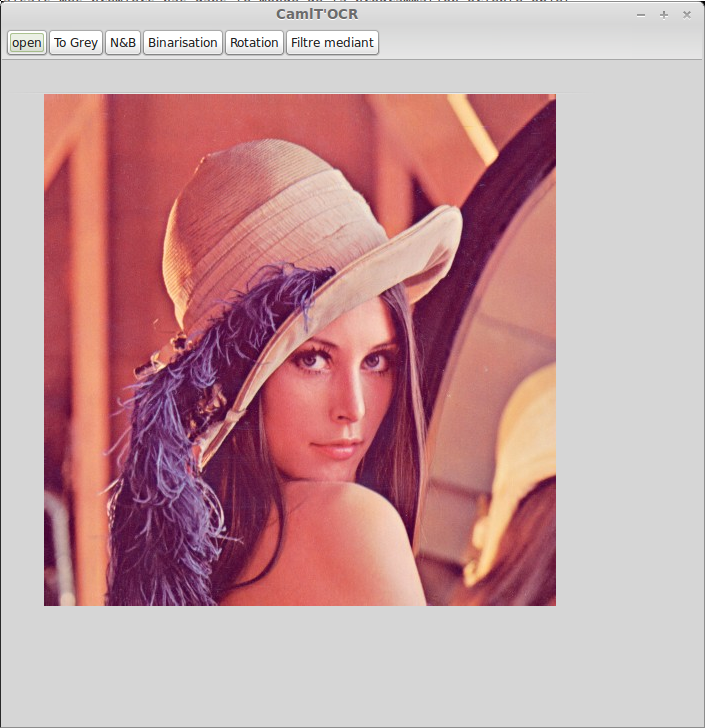
\includegraphics[width=0.80\textwidth]{gui.png}
	 \label{Dernier GUI}
\end{figure}
\\
- une barre de menus déroulants permettant d’avoir accès à toutes les fonctions importantes
du logiciel, réparties en diverses catégories.\\
- un cadre réservé à l’image à traiter et un cadre réservé à l’image après le traitement.
Il est possible d’ouvrir une image à partir d’une fenêtre de sélection de fichiers en cliquant
sur « Ouvrir » dans le menu Fichier. Celle-ci est importée à sa taille réelle et si
l’image est trop grande, l’utilisateur s’aidera des barres de défilement.
- des bouttons de fonction précise pour le traitement de l’image :\\
	- Niveau de gris : on transforme l'image colorée en niveau de gris afin de pouvoir   utiliser la fonction Noir et Blanc de manière plus efficace.\\
	- Noir et Blanc : on tranforme l'image colorée ou en niveau de gris en noir et blanc.\\
	- Filtrage : on applique un filtre à l’image pour améliorer sa qualité et enlever les impuretés.\\
	- Rotation : on utilise cette fonction si l'image importée a une inclinaison afin de lui  faire une rotation pour la rendre droite.\\
	- Détection des lignes : on utilise cette fonction pour détecter les lignes de texte de l'image.\\
	- Détection des lettres : on utilise cette fonction pour détecter chaque bloc de 	caractère de l'image.\\
	- Analyse : cette fonction finale vous fait un rendu dans un fichier texte du texte extrait  de l'image \\
- une barre de progression permettant à l’usager de visionner la progression de l’application
en cours.\\




              \subsection{Aspect technique}
\textbf{Chargement et sauvegarde de l'image :}\\
Nous avons rajouté le chargement et la sauvegarde de l’image qui sont indispensables à l’utilisation du logiciel. Il a donc fallu manipuler deux propriétés essentiels : OpenFileDialog et SaveFileDialog. Ces deux propriétés ont permettent respectivement de créer une fenêtre d’exploration (pour importer l’image) et une fenêtre de sauvegarde (pour enregistrer l’image sous).\\

              \subsection{Redimensionnement de l'image}
Le traitement de l’image représente uen partie essentielle pour le fonctionnement de l’OCR. Pour une bonne utilisation et surtout une présentation visuellement agréable du logiciel, il est indispensable de redimensionner l’image que l’on traite.
Bien que nous ayons finalisé la détection des blocs et des lignes de textes jusqu’aux blocs de caractères, nous sommes encore loin de qualifier notre logiciel d’OCR, c’est pourquoi le logiciel a pour seul but de traiter une image et d’en donner un apercu. Pour cela, l’interface a besoin de deux PictureBoxs (litteralement deux "boites d’image", une pour l’image a traiter et une pour l’apercu de l’image apres traitement). 
Lorsque l’on importe une image dans une PictureBox, la PictureBox prend la dimension de l’image qu’elle contient. On veut afficher deux images cote a cote de meme dimension et l’inconvenient serait qu’elles soient trop grandes pour etre affichees entièrement dans l’ecran. Voici un exemple :\\
\begin{figure}[hp]
	\centering
    \includegraphics[width=0.80\textwidth]{badim.jpg}
	 \label{Mauvaise redimension}
\end{figure}
\\
Pour remedier a ce probleme, il faut justement redimensionner l'image. Pour que
les deux images s'affichent entierement on a restreint les dimensions de l'image, en
d'autres termes on lui a donne une taille maximale du champ dans lequel il peut s'afficher.\\

Cependant, le redimensionnement de l'image doit respecter plusieurs proprietes :
- l'image doit conserver ses proportions.\\
- la taille maximale des PictureBoxs doit s'adapter a n'importe quel type d'ecran.
Pour une redimension parfaite, il a fallu gerer 4 cas.\\
Le premier cas est lorsque la dimension de l'image importee est plus petite que la taille
maximale de la PictureBox1. C'est le cas le simple car on a pas besoin de redimensionnement.\\

Le deuxieme et troisieme cas sont similaires. C'est lorsque la hauteur de l'image depasse
la hauteur de la taille maximale de la PictureBox1 (ou dans l'autre cas, la largeur
de l'image depasse la largeur de la taille maximale de la PictureBox1).\\
\begin{figure}[hp]
	\centering
    \includegraphics[width=0.70\textwidth]{difcas.jpg}
	 \label{differents cas.}
\end{figure}
\\
Le redimensionnement sera donc different selon ces conditions afin d'obtenir une affichage
optimale de l'image. De plus, grace a la propriete Screen.PrimaryScreen, la
taille maximale de la PictureBox est calculee en fonction de la taille de l'ecran. Les
proportions seront donc respectees sur tout type d'ecran. Le resultat donne ceci :\\
\begin{figure}[hp]
	\centering
    \includegraphics[width=0.80\textwidth]{result.png}
	 \label{Redimesnionement}
\end{figure}
\newpage
\\

              \subsection{Exceptions}
Pour éviter tout incident ou bug lors de l’utilisation du logiciel, nous avons eu à
gérer des exceptions sans lesquelles il serait problématique d’avoir une liberté totale dans l’utilisation. Les trois exceptions les plus récurrentes sont les suivantes :
- Utiliser une des fonctions sans image.\\
- Importer un fichier d’un format autre que Bitmap, JPG, JPEG, PNG ou GIF.\\
- Entrer une adresse IP et un port invalides lors de la sauvegarde à distance.\\

\begin{figure}[hp]
	\centering
    \includegraphics[width=0.80\textwidth]{exeption1.png}
	 \label{Exception}
\end{figure}
\\
\begin{figure}[hp]
	\centering
    \includegraphics[width=0.80\textwidth]{exeption2.png}
	 \label{Exception}
\end{figure}
\\
\newpage
\begin{figure}[hp]
	\centering
    \includegraphics[width=0.80\textwidth]{exeption3.png}
	 \label{Exception}
\end{figure}\\

Ainsi notre interface graphique se constitue pour l’instant d’éléments simples, utiles
et efficaces.


      \section{Traintement de l'image }
              \subsection{Filtrage et binarisation }
                          \subsubsection {Binarisation d'une image : niveau de gris}

\textbf{La théorie :}\\
Une image est composée de pixels, chacun de ces pixels sont d’une certaine couleur. La couleur varie selon plusieurs composantes, le niveaux de rouge ( R ), le niveau de vert (G) et le niveau de bleu (B) mais aussi parfois le canal alpha qui correspond à la transparence du pixel noté A, il ne nous est pas utile pour le moment mais on ne sait jamais, mieux vaut le savoir. Ces composantes sont des entiers compris entre 0 et 255. Pour transformer une image en niveaux de gris il faut récupérer les trois composantes du pixel (R.G.B) et en faire une moyenne. Ainsi on obtient une valeur comprise entre 0 et 255 cette valeur doit alors être remplacée dans chaque composante du pixel. Et voilà c’est aussi simple que ça !
\\

\textbf{Le principe de mon algorithme :} \\
Une fois la théorie comprise, l’algorithme est très simple à concevoir car il suit exactement les étapes citées ci-dessus. Premièrement, l’algorithme prend en paramètre une image (celle que nous voulons traiter) puis il encrée une nouvelle (vierge) selon les même dimensions. Ensuite, il va parcourir chaque pixel de l’image à traiter, récupérer ses composantes, en faire la moyenne et créer un  nouveau pixel qui sera mis à la même position dans l’image vierge avec ses composantes égales à la valeur de la moyenne trouvée précédemment.
\newpage
\\
    \begin{figure}[hp]
	    \centering
	    \includegraphics[width=0.80\textwidth]{image1.jpg}
	    \caption{Niveau de gris}
    \end{figure}
\\

                          \subsubsection {Binarisation d'une image : noir et blanc}
\textbf{La théorie :}\\
Pour le passage en noir et blanc, il faut utiliser l’image mise en niveau de gris. L’utilisation d’un seuil (calculé mathématiquement) est requise pour parvenir à la réalisation de cette étape. Une fois le seuil trouvé il suffit de comparer chaque pixel en niveau de gris par rapport au seuil, si la valeur d’une des composantes du pixel est inférieure au seuil alors on définit la couleur du pixel comme étant noir, on la définit en blanc dans le cas inverse.
\\

\textbf{Le principe de mon algorithme :} \\
Cet algorithme prend donc une image mise en niveaux de gris comme paramètre. De la même manière que lors de l’algorithme précèdent, une nouvelle image va être crée, l’image en niveau de gris va être parcourue puis l’une des composantes de chaque pixel va être récupérée (une seul composante car les trois ont la même valeur). Vient ensuite l’étape du calcul du seuil. Pour cela, l’algorithme parcourt les pixels à proximité du pixel actuel (un rang avant et un rang après en x et en y), récupère une des composantes et la stocke dans une liste (donc une liste de neufs valeurs avec celle du pixel actuel). Il suffit maintenant de trouver la valeur maximale et la valeur minimale contenue dans cette liste puis d’en faire une moyenne et ainsi la comparer à la couleur du pixel de l’image mise en niveau de gris, si la couleur est inférieure au seuil alors on place un pixel noir à la même position dans l’image vierge, inversement dans le cas inverse.
\newpage
\\
    \begin{figure}[hp]
	    \centering
	    \includegraphics[width=0.80\textwidth]{image2.png}
	    \caption{binarisation}
    \end{figure}
\\
\\
                          \subsubsection {Filtres : généralitées}
La mise en place de filtres (eh oui il y en a plusieurs !) est une étape très importante dans la réalisation d’un OCR car ce sont eux qui sont responsables d’améliorer la qualité de l’image (enlever toutes les impuretés pouvant entraîner une erreur dans l’analyse des caractères mais aussi augmenter le contraste de chaque lettre pour aider la reconnaissance et bien d’autres encore !).\\

Pour ce qui est de la mise en place de filtres dans notre projet, j’ai réalisé deux filtres permettant d’enlever le bruit de l’image (c’est-à-dire enlever tout pixel parasite). La
binarisation faisant déjà une bonne partie du travail, l’application de filtre n’est nécessaire que si l’image est vraiment très bruitée comme ça par exemple :\\
\newpage
    \begin{figure}[hp]
	    \centering
	    \includegraphics[width=0.80\textwidth]{imagetest.jpg}
	    \caption{Maison bruite}
    \end{figure}
\\
Les filtres que j’ai implémentés sont le filtre moyenne et le filtre médian. Le deuxième étant bien plus efficace que le premier c’est la raison pour lequel il sera présenté durant la soutenance.

                          \subsubsection {Filtres : Le filtre moyenneur}
Ce filtre est un filtre de réduction de bruit et de lissage d’une image, comme son nom l’indique, il utilise la moyenne des couleurs des pixels à proximité du pixel cible et remplace la couleur du pixel cible par cette moyenne. L’inconvénient de ce filtre est qu’il a tendance à trop lisser les contours présents dans un image ce qui peux poser des problèmes lorsque l’image à traiter est un scan de texte car chaque caractère risque de se retrouver collé au caractère suivant ou au précèdent (voir même aux deux).\\
\newpage
    \begin{figure}[hp]
	    \centering
	    \includegraphics[width=0.80\textwidth]{moy.jpg}
	    \caption{Filtre moyenneure.}
    \end{figure}
                          \subsubsection {Filtres : le filtre m�diant}
Ce filtre est essentiellement un filtre de réduction de bruit, il a pour vocation de supprimer les pixels isolés en les remplaçant par la valeur médiane des pixels à proximité. Pour ce faire, chaque valeur d’une composante des pixels alentours doit être stockée dans une liste, la liste doit être triée par ordre croissant ainsi la valeur médiane (valeur qui coupe la liste en deux partie égales) peut être facilement trouvée en divisant la liste par deux.\\
    \begin{figure}[hp]
	    \centering
	    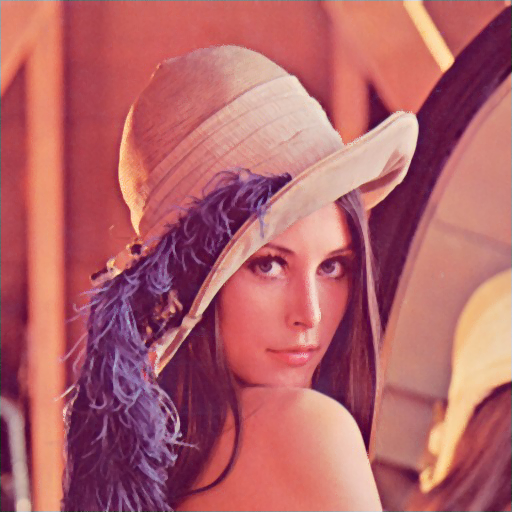
\includegraphics[width=0.80\textwidth]{median.jpg}
	    \caption{Filtre median}
    \end{figure}
\\

              \subsection{Rotation de l'image }
                          \subsubsection {la detection de l'angle et la rotation}
\textbf{La transformée de Hough :}\\
C est ici que l on commence à prendre plaisir Je me suis donc occupé de la transformée de Hough. La transformée de Hough est une technique de reconnaissance de formes inventée en 1962 par Paul Hough. Le principe qui sous-tend la transformée de Hough est qu’il existe un nombre infini de lignes qui passent par un point, dont la seule différence est l’orientation (l’angle). La transformée généralisée de Hough fonctionne sur le même principe que la transformée de Hough : on recherche la présence d’une courbe, caractérisée par un certain nombre de paramètres ; chaque point de l’image analysée « vote » pour l’ensemble des jeux de paramètres générant des courbes auxquelles il appartient. La présence d’une courbe recherchée est caractérisée par un jeu de paramètres ayant un score élevé. Je me suis servi de cette méthode pour trouver un angle de rotation, de manière automatique au cas où une image rentrée en paramètre soit inclinée. Une droite peut s écrire de différente manière : y = ax+b mais aussi T = x.cos(teta) * y.sin(teta). Pour un même angle, tous les points dune droite on exactement le même T. En calculant la valeur de T de chaque pixel noir, pour un angle teta, (variant ici de -30 a +30 degrés avec un pas de 0,01) , et en attribuant un incrément dans un tableau au couple (droite/angle) alignant le plus de pixel noir, on peut déduire assez facilement quel est l angle le plus récurrent ainsi trouvé. La valeur de l angle correspond néanmoins pas à l angle de rotation de limage. Pour le trouver on fait teta pi/2.
\\
    \begin{figure}[hp]
	    \centering
	    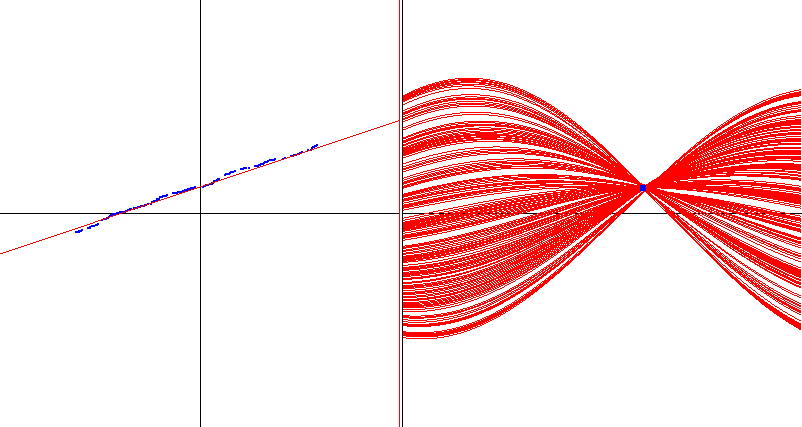
\includegraphics[width=0.80\textwidth]{hough.jpg}
	    \caption{hough}
    \end{figure}
\\

                          \subsubsection {Les problèmes rencontrés}
J ai rencontré plusieurs problèmes lorsque j ai implémenté l algorithme. La simple compréhension ne fut pas simple, mais une fois comprise on comprend bien que ce n'est pas si dur que cela. J ai eu d abord des problèmes d optimisation : programme long à compiler. J ai réduit l angle d étude (qui était de 180 degrés) à une tranche entre -30 et 30 degrés. J ai eu un autre problème, c est la perte de précision lors du passage des ints au doubles ou aux floats. J ai choisi de tronquer certains résultats en int pour gagner du temps mais parfois au prix dune perte de précision. Car en effet l angle teta obtenu est en radiant et il faut le reconvertir en degré. D où l importance des dixièmes et des centièmes de radiant pour la précision !\\
\\
    \begin{figure}[hp]
	    \centering
	    \includegraphics[width=0.80\textwidth]{pi.jpg}
	    \caption{Approximation}
    \end{figure}
\\
J'ai travaillé en degré et non pas en radiant car le Framework propose une méthode de rotation, mais qui nécessite de prendre un angle de rotation en paramètre qui soit en degré. Il y a eu aussi une perte de qualité dimage lors de la rotation qui fut réglée via une autre méthode du Framework !!\\
\newpage
    \begin{figure}[hp]
	    \centering
	    \includegraphics[width=0.60\textwidth]{micronet.jpg}
	    \caption{Framewrok}
    \end{figure}
\\
              \subsection{Segmentation de l'image }
                          \subsubsection {Détection des lignes}
La segmentation des lettres est un traitement visant à isoler chaque caractères afin de pouvoir l’envoyer au réseau de neurone pour la reconnaissance. Ce traitement ce décompose en plusieurs étapes, premièrement il faut détecter chaque bloc de texte (paragraphes) présents sur l’image. Ensuite dans chacun de ces blocs il faut repérer chaque lignes, puis pour chaque ligne isoler chaque caractères.\\

L’algorithme que j’ai mis en place permet directement de detecter les lignes, pour ce faire il parcours horizontalement les pixels de l’image en commencant par le haut de celle ci. Le premier pixel noir trouvé represente alors la limite superieur d’une potentielle ligne. A partir de ce stade, je continue ma recherche horizontale sur la ligne en dessous de la limite superieur en ayant implémenté une variable de hauteur qui va être incrementée l orsqu’un pixel de couleur noir est trouvé. Des qu’il est trouvé l’algorithme passe a la ligne suivante, et ainsi de suite jusqu’à ce que le parcours finisse sur le bord droit de l’image sans avoir trouvé de pixels. Il ne reste plus qu’a detecter les limites droites et gauches de ces lignes. Nous avons donc la limite superieur et inférieur de la ligne en question, pour trouver les bordures il suffit de parcourir verticalement les pixels contenus entre les limites de la ligne puis de retourner la position du premier pixel trouvé. Pour cela il y a deux algorithmes, le premier parcours l’image
en partant du bord gauche de celle ci, le deuxieme est le meme a l’exception qu’il part du bord droit de l’image. La detection d’une ligne est donc finie ! ! a partir de ce stade l’algorithme recommence ses operations en partant de la limite inferieur de la ligne et ce jusqu’à ce qu’il arrive en bas de l’image. Au final, lorsque l’algorithme est terminé, il renvois une liste de rectangle representant les lignes ainsi on a la position exact la longueur et la largeur de chacune d’elles.\\

. \\
   \begin{figure}[hp]
	    \centering
	    \includegraphics[width=1.10\textwidth]{lignes.jpg}
	    \caption{Detection des Lignes}
    \end{figure}
\\

                          \subsubsection {Détection des caractères}
Pour la détection des caractères, j’ai implémenté un autre algorithme qui se base
sur le résultât de la détection des lignes. C’est a dire qu’il ne travail que sur la liste
de rectangle retourné par la recherche des ligne. L’algorithme est simple il parcours
verticalement l’image contenue dans le rectangle, lorsqu’un pixel noir est trouvé il
initialise une variable a cette position puis il continue sur la ligne verticale suivante
jusqu’à ce qu’il finisse sur la limite inférieur du rectangle quand il n’a pas trouvé de
pixel. A cette position il initialise une autre variable qui permettra de définir la largeur
du rectangle contenant la lettre une fois la lettre segmentée il ajoute ce rectangle dans
une liste et continue son parcours jusqu’à la bordure droite du rectangle de ligne. Puis
effectue la même action sur chacun des rectangles contenus dans la liste de ligne.
\newpage
\\
   \begin{figure}[hp]
	    \centering
	    \includegraphics[width=1.10\textwidth]{lettres.jpg}
	    \caption{Detection des caractères}
    \end{figure}
\\
\\
   \begin{figure}[hp]
	    \centering
	    \includegraphics[width=0.90\textwidth]{zoom.png}
	    \caption{Detection des caractères (zoom)}
    \end{figure}
\\

       \section {La reconnaissance de caractère}
                \subsection{Introduction au réseau de neurones }
Tout d’abord, ce que l’on désigne habituellement par "réseau de neurones" est en fait un réseau de neurones artificiels basé sur un modèle simplifié de neurone. Ce modèle permet certaines fonctions du cerveau, comme l’apprentissage par l’exemple, le travail en parallèle, mais le neurone artificiel est loin de posséder toutes les capacités du neurone biologique. Les réseaux de neurones biologiques sont ainsi beaucoup plus compliqués que les modèles mathématiques et informatiques. \\

Il n’y a pas de définition universellement acceptée de "réseau de neurones". On considère généralement qu’un réseau de neurones est constitué d’un grand ensemble d’unités. (ou neurones), ayant chacune une petite mémoire locale. Ces unités sont reliées par des canaux de communication (les connexions, aussi appelées synapses d’après le terme biologique correspondant), qui transportent des données numériques. Les "unités" peuvent uniquement agir sur leurs données locales et sur les entrées qu’elles reçoivent par leurs connexions.\\

Certains réseaux de neurones sont des modèles de réseaux biologiques, mais d’autres ne le sont pas. Historiquement l’inspiration pour les réseaux de neurones provient cependant de la volonté de créer des systèmes artificiels sophistiqués, voire "intelligents", capables d’effectuer des opérations semblables à celles que le cerveau humain effectue de manière routinière, et d’essayer par là d’améliorer la compréhension du cerveau. La plupart des réseaux de neurones ont une certaine capacité d’apprentissage. Cela signifie qu’ils apprennent à partir d’exemples, de même que les enfants apprennent à distinguer les chiens des chats à partir d’exemples de chiens et de chats. Le réseau peut ensuite dans une certaine mesure être capable de généraliser, c’est-à-dire de produire des résultats corrects sur des nouveaux cas qui ne lui avaient pas été présentés au cours de l’apprentissage.\\

Les réseaux de neurones, structures artificielles de neurones, constituent une approche permettant d’aborder sous des angles nouveaux les problèmes de perception, de mémoire,
d’apprentissage et de raisonnement. Ils s’avèrent également des alternatives très prometteuses pour contourner certaines des limitations des ordinateurs classiques.\\

Les réseaux de neurones servent aujourd’hui a toutes sortes d’applications dans un grand nombre de domaines. En effet ont été developpés, par exemple, un système de guidage pour automobile, des systèmes de lecture automatique de chèques bancaires et d’adresses postales, des sytèmes de traitement du signal pour différentes applications militaires. . .\\

Parmi tous ces développements on ajoutera également l’OCR qui utilise ces réseaux pour apprendre et minimiser, par apprentissage, les erreurs commises lors de la lecture des documents. Bref ! Les réseaux de neurones ont un impact considérable de nos jours et il y a fort à parier que leur importance ne cessera de croitre dans le futur.\\


                \subsection{Modèle de neurone et réseau }
Principe : le réseau doit être facilement et entièrement reconfigurable, afin de pouvoir tester rapidement de nouvelles architectures sans avoir à tout reprogrammer. Par exemple, il est immédiat de modifier le nombre de neurones d.une aire donnée (une assemblée particulière de neurones ; ce sera précisé un peu plus loin), de l.interconnecter à toute autre aire, de créer des boucles de rétroaction, ou de modifier des filtres.\\
\newpage
    \begin{figure}[hp]
	    \centering
	    \includegraphics[width=0.80\textwidth]{modeleNN.png}
	    \caption{Modèle de réseau de neurones }
    \end{figure}
\\
Un neurone artificiel est répresente par le modèle mathematique de la figure ci-dessus. Un neurone est essentiellement constitue d’un integrateur qui effectue la somme pondérée de ses entrées. Le résultat n de cette somme est ensuite transformé par une fonction de transfert f qui produit la sortie a du neurone.
La sortie n correspond a une somme pondérée des poids et des entrées moins ce qui est nomme le biais b. Le résultat n de la somme pondérée est appelé niveau d’activation du neurone. Le biais b s’appelle aussi le seuil d’activation du neurone. Lorsque le niveau
d’activation atteint ou dépasse le seuil b, alors l’argument de f devient positif ou nul.\\
Sinon, il est négatif.\\

Un poids d’un neurone artificiel représente, en faisant le parallèle avec de vrais neurones, a l’efficacité d’une connexion synaptique. Un poids négatif vient alors inhiber une entrée tandis qu’un poids positif vient l’accentuer. Il subsiste tout de même un facteur limitatif dans le modèle énoncé précédemment. En effet, pour pouvoir simuler un réseau de neurones on va considérer le temps comme étant discret dans les équations., i.e considérer que tous les neurones sont synchrones. Cependant dans les modèles biologiques les neurones sont asynchrones. Ceci nous amène donc à considérer le modèle matriciel ci-dessous.\\
\newpage

\\
    \begin{figure}[hp]
	    \centering
	    \includegraphics[width=0.80\textwidth]{modeleMA.png}
	    \caption{Modèle de réseau de neurones (2) }
    \end{figure}
\\
On introduit alors un un schéma plus compact du modèle presénté précédemment. Les R entrées sont représentées par un rectangle noir (le nombre d’entrées étant indiqué sous le rectangle). De ce rectangle sort le vecteur p de dimension matricielle R x 1. Ce vecteur est multiplié par une matrice W qui contient les poids (synaptiques) des neurones (dans le cas d’un neurone simple la matrice W est de dimension R x 1). Le résultat de cette multiplication correspond au niveau d’activation qui est ensuite comparé au seuil b, qui est un scalaire, par soustraction. Enfin, la sortie du neurone est calculée par une fonction d’activation f et le résultat obtenu est un scalaire.\\

\textbf{Fonction de transfert :}
Il existe plusieurs possibilité concernant la nature de la fonction d’activation pour le modèle présenté précédemment. Différentes fonctions de transfert peuvent alors être utilisées en tant que fonction d’activation du neurone. Parmi les plus communément utilisées on trouve la fonction "seuil", la fonction "lineaire" et la fonction "sigmoide". Concernant la fonction seuil, celle-ci applique, comme son nom l’indique, un seuil à l’entrée du neurone. Une entrée négative ne passe pas le seuil, la fonction retourne 0 (faux), alors qu’une entrée positive ou nulle dépasse le seuil et la fonction retourne 1 (vrai).Parmi les autres fonctions de transfert on trouve la fonction seuil symétrique, linéaire saturée,linéaire saturée symétrique, linéaire positive, tangente hyperbolique ou encore compétitive.
\newpage
    \begin{figure}[hp]
	    \centering
	    \includegraphics[width=0.50\textwidth]{modeleAA.png}
	    \caption{Architecture du reseau}
    \end{figure}

\\
Un réseau de neurones est en réalite un maillage de neurones, généralement organisé en couches. Afin de construire une couche de S neurones, il suffit simplement de les assembler comme sur la figure ci-dessus. Les S neurones d’une même couche sont tous reliés aux R entrées, la couche est alors dite entièrement connectée. Un poids wi ;j est associé à chacune des connexions et désigne le poids de la connexion qui relié le neurone i à son entrée j. Finalement, pour construire un réseau, il ne suffit plus que de combiner des couches de neurones. La dernière couche est dite "couche de sortie" et les couches précédentes "couches cachees" Les réseaux multicouches sont beaucoup plus puissants que les réseaux simples à une seule couche. Sauf dans de rares cas, les réseaux de neurones artificiels exploitent deux ou trois couches. Il sera également nécessaire d’entrainer ce réseau, c’est-à-dire modifier la valeur de ses poids et de ses biais pour qu’il réalise la fonction entrée / sortie désirée.
\newpage

\\
    \begin{figure}[hp]
	    \centering
	    \includegraphics[width=0.80\textwidth]{modeleMA2.png}
	    \caption{Modèle de réseau de neurones (3)}
    \end{figure}
\\
\\
    \begin{figure}[hp]
	    \centering
	    \includegraphics[width=0.80\textwidth]{modeleMA3.png}
	    \caption{Modèle de réseau de neurones (4)}
    \end{figure}
\\

                \subsection{Processus d'apprentissage }
Parmi l’ensemble des propriétés d’un réseau de neurones, la plus fondamentale de toutes est celle relative à la capacite d’apprendre de son environnement, d’évoluer et d’améliorer sa performance au travers d’un processus d’apprentissage. L’apprentissage peut se définir comme suit.
L’apprentissage est un processus dynamique et iteratif permettant de modifier les paramètres
d’un réseau en réaction avec les stimuli qu’il recoit de son environnement. Le type d’apprentissage est déterminé par la manière dont les changements de paramètres surviennent.
De cette définition découle alors la nécessite d’une stimulation du réseau par un environnement.
Ce dernier doit alors évoluer en conséquence, subir un certain nombre de changements qui seront répercutes dans le futur lors d’une nouvelle interaction avec l’environnement. L’apprentissage se fait alors par modification de l’efficacité synaptique, i.e par un changement dans la valeur des poids qui relient les neurones d’une couche à une autre.


\textbf{Par correction de l'erreur :}\\

La première règle que l’on peut utiliser pour l’apprentissage est fondée sur la correction
d’erreurs observées.\\
Soit ai(t) la sortie que l’on obtient au temps t pour le neurone i. Cette sortie résulte d’un stimulus p(t) que l’on applique aux entrées du réseau dont un des neurones correspond au neurone i. Soit di(t) la sortie que l’on désire obtenir au temps t pour le neurone i. ai(t) et di(t) sont généralement différents d’ou l’on cherche à calculer l’erreur ei(t) en soustrayant ai(t) a di(t). Il est bien évident que l’on cherche à réduire au maximum cette erreur. La règle de la correction de l’erreur est très répandue dans les réseaux de neurones artificiels, bien qu’elle ne soit pas plausible biologiquement. De plus celle-ci ne peut être utilisée que dans un contexte d’apprentissage supervisé.\\


\textbf{Par la régle de Hebb :}\\

Cette règle s’inspire des travaux réalisés par le neurophysiologiste Donald Hebb.
Dans le contexte des réseaux artificiels ce règle s’énonce en deux parties :\\

1. Si deux neurones de part et d’autre d’un synapse sont activés simultanement, alors la force de ce synapse doit être augmentée;
2. Si deux neurones identiques sont activés de manière asynchrone, alors le synapse
correspondant doit être affaibli ou carrément éliminé.\\

Un tel synapse est donc dit "synapse hebbien". Il utilise un mécanisme interactif, dépendant
du temps et de l’espace, pour augmenter l’efficacité synaptique d’une manière proportionnelle à la correlation des activites pré- et post-synaptiques. \\


\textbf{Compétitif  :}\\

L’apprentissage compétitif consiste à organiser une compétiton entre les neurones d’un réseau pour savoir lequel sera actif à un instant donné. Contrairement aux autres types d’apprentissage ou les neurones peuvent apprendre simultanément et de la même manière, l’apprentissage compétitif a pour objectif de produire un "vainqueur" et, dans certains cas, un ensemble de neurones "voisins" du vainqueur. Des lors seuls le vainqueur et, potentiellement, son voisinage bénéficient d’une adpatation de leur poids. L’apprentissage est alors dit local car il est limite à un sous-ensemble des neurones du réseau.\\

Ainsi, les neurones individuels peuvent apprendre a se specialiser sur des sous-ensembles de stimuli similaires pour devenir des détecteurs de caractéristiques.
L’apprentissage compétitif est surtout utilisé dans le contexte d’un apprentissage non
supervisé, i.e lorsque l’on ne connaît pas les valeurs desirées pour les sorties du réseau.\\


\textbf{Supervisé :}\\
L’apprentissage supervisé est caractérisé par la présence d’un "professeur" qui possède une connaissance approfondie de l’environnement dans lequel évolue le réseau de neurones. Le connaissances du professeur prennent, en pratique, la forme d’un ensemble de Q couples de vecteurs d’entrée et de sortie note f (p1 ; d1), ... , (pQ ; dQ) g, ou pi désigne un stimulus (une entrée) et di la cible pour ce stimulus, i.e les sorties desirées pour le réseau. De ce fait l’apprentissage supervisé est aussi qualifié d’apprentissage par des exemples. L’apprentissage supervisé n’est rien d’autre qu’un synonyme pour l’apprentissage par correction d’erreurs et possède de facto les même limitations. En effet, sans la présence d’un professeur pour fournir les valeurs cibles, le réseau ne peut en aucun cas apprendre de nouvelles stratégies pour de nouvelles situations qui ne sont pas couvertes par les exemples d’apprentissage.**


\textbf{Par renforcement :}\\
L’apprentissage par renforcement permet de contourner certaines limitations de l’apprentissage supervisé. Il ressemble à l’apprentissage supervisé excepté qu’il possède un indice de satisfaction scalaire au lieu d’un signal d’erreur vectoriel. Cette méthode est basée sur les travaux en psychologie expérimentale de Thorndike. Dans le contexte des réseaux de neurones artificiels, l’énoncé de Thorndike peut être reformulé comme suit :\\
lorsqu’une action (decision) prise par le reseau engendre un indice de satisfaction positif, alors la tendance du réseau à prendre cette action doit être renforcée. Autrement, la tendance à prendre cette action doit être diminuée. En pratique la mise en oeuvre de ce type d’apprentissage est particulièrement complexe.


\textbf{Non-supervisé :}\\
La dernière forme d’apprentissage est l’apprentissage dit "non-supervisé" ou encore "auto-organisé". Celui-ci est caracterisé par l’abscence complète de tout professeur, ce qui induit l’abscence d’un signal d’erreur, comme dans l’apprentissage supervisé, ou encore d’un indice de satisfaction dans le cas d’un apprentissage par renforcement. 
Des lors on ne dispose que d’un environnement qui fournit des stimuli au réseau. En assimilant les stimuli de l’environnement à une description de son état interne, la tâche du réseau est alors de modéliser cet état du mieux possible. A la fin de l’apprentissage le réseau a developpé une habilité à former des représentations internes des stimulis de l’environnement permettant d’encoder les caractéristiques de ceux-ci et par conséquent de créer automatiquement des classes de stimuli.


                \subsection{Perceptron multicouche}
Parmi les différents types de réseaux de neurones on trouve le "perceptron multicouche" (PMC). Ce type de réseau est dans la famille générale des réseaux dit à "propagation par l’avant", i.e que lors d’une utilisation normale l’information se propage dans un sens unique, des entrées vers les sorties sans aucune rétroaction. Son apprentissage est de type supervisé, par correction des erreurs. dans ce cas uniquement le signal est "rétropropage" vers les entrées pour mettre à jour les poids des neurones. Le perceptron multicouche est un des réseaux de neurones les plus utilisés pour des problèmes d’approximation, de classification et de prédiction. Il est habituellement constitué de deux ou trois couches de neurones totalement connectés. Il n’est donc rien d’autre qu’un assemblage de couches concaténées les unes aux autres, de la gauche vers la droite, en prenant les sorties d’une couche et en les injectant comme les entrées de la couche suivante. De plus l’algorithme dit de "rétropropagation des erreurs" permet d’entrainer ce type de réseau en modifiant les poids à partir de la couche de sortie vers les couches antérieures.
       \section {La recherche }
Pour la soutenance, je me suis principalement occupé de la recherche de mot clef dans un dictionnaire.Plus précisément, avec le mot en sortie du réseau de neurone, je devais essayer, à l’aide d’un dictionnaire,de trouver le mot français correspondant. J’ai donc dans un premier temps utilisé l’algorithme de Levenshtein pour établir la distance de Levenshtein.
                \subsection{Levenshtein}
Cette algorithme permet de trouver un entier qui correspondra au nombre de changement de lettre qu’il faudra pour aller d’un mot X, vers un mot Y. C’est assez simple , et je vais vous expliquer avec un exemple. Prenons l’exemple basique : Le mot du réseau de neurone sera "chiens" et un des mots de notre dictionnaire sera "niche". On va donc établir une matrice dite de "coût" avec les deux mots. En abscisse le mot du réseau de neurone et en ordonné, le mot que l’on recherche.\\
Si la lettre en abscisse correspond à une lettre en ordonné on met un zéro dans la matrice de coût, sinon on ajoute un 1, pour obtenir au final cette matrice :

    \begin{figure}[hp]
	    \centering
	    \includegraphics[width=0.80\textwidth]{m1.jpg}
	    \caption{Matrice de cout}
    \end{figure}
\\
On établit ensuite une deuxième matrice, celle qui va nous permettre d’établir la distance de Levenshtein. On met en abscisse la longueur du mot CHIENS +1, et en ordonné la longueur du mot de notre dictionnaire+1 , ici NICHE +1. On obtient donc la matrice suivante :\\
\newpage
    \begin{figure}[hp]
	    \centering
	    \includegraphics[width=0.80\textwidth]{m2.png}
	    \caption{Matrice de Levenshtein}
    \end{figure}
\\
Il va falloir maintenant remplir les cases vides, d’une manière bien spécifique. Prenons le schéma suivant :\\
    \begin{figure}[hp]
	    \centering
	    \includegraphics[width=0.80\textwidth]{MA4.png}
	    \caption{Distance de Levensthein}
    \end{figure}
\\
Nous allons utiliser un procédé récursif. Pour savoir ce qu’on obtiendra dans la case (1 ; 1), on fait le minimum entre trois différentes valeurs. Soient x,y,z les trois valeurs.\\
x = valeur case verte +1 ;\\
y = valeur case bleu +1 ;\\
Pour z, il faut ce référer à la matrice de coût. Si la valeur de l’équivalent de la case rouge dans la matrice de coût est égale à 1 , alors z = valeur de case rouge +1 ; si la valeur de l’équivalent de la case rouge dans la matrice de coût est égale à 0, alors z = valeur de la case en rouge.
On applique cette même idée sur toute les cases du tableau.\\
Une fois qu’on est à la case (6 ; 5), alors on applique le procédé une dernière fois.\\
Et dans cette dernière case , on obtient la distance de Levenshtein. Plus elle est grande, plus cela veux dire que les mots sont différent. Si elle est nul, on considère que les deux mots sont identiques, si elle est égale à 1, cela veut dire que les mots ont une lettre de différence.

NB : lorsqu’il y a écrit CHIEN et NICHE dans les schéma/tableau, ce ne sont bien évidemment que des indications pour mieux comprendre, et appliquer le procédé en lui-même, ce ne sont pas deux chaînes de caractère qui sont dans une matrice d’entier.\\



                \subsection{Le Dictionnaire}
Dans un second temps, il fallait effectué une recherche dans un dictionnaire. C’est-à-dire faire l’analogie entre le mot que le réseau de neurone va nous sortir, et les mots du dictionnaire. . \\
Prenons un exemple :

Si le réseau de neurone nous sort le mot : "Bongour" qui n’existe pas dans la langue française, nous devons recherche un mot dans le dictionnaire, avec la distance de Levenshtein la plus faible.
Quand bien même, le mot du réseau de neurone serait "Bonjour", il nous faudrait chercher
dans le dictionnaire si ce mot existe.\\
Mais la recherche dans un dictionnaire est assez longue si on parcourt séquentiellement\\
le dictionnaire, et que celui-ci est très gros (+300 000 mots par langue par exemple). Il nous a fallut trouver une astuce. Le mot donné par le réseau de neurone comporte potentiellement des erreurs. La première lettre peut ne pas être la bonne. On ne peut donc pas se fier à la première lettre pour faire un tri dans le dictionnaire : si le mot du réseau de neurone commence par "a", on ne peut donc pas chercher seulement parmis les mots qui commence par "a".J’ai donc choisi une autre méthode de tri. Le dictionnaire va être "sous-trié". Si le mot issu du réseau de neurone contient 5 caractères. On crée un sous-dictionnaire de tout les mots de 5 caractères et on ne cherche que dans le sous dictionnaire. La recherche effectuée est donc plus rapide. Car l orsqu’on crée le sous-dictionnaire, on ne compare que des entiers (la taille du mot), alors que lors de la recherche, on se sert de tout le procédé de Levensthein qui a une complexité qui dépend de la taille du mot.\\
On crée le sous dictionnaire dans un petit fichier ".txt", via les stream du c. En moyenne, sur notre dictionnaire actuelle (63050 mots), on fera l’algorithme de Levensthein sur 9000 mots au plus, et en moyenne sur 5000 mots. \\
Je me suis aussi occupé de toute l’implémentassions de la recherche dans le Winform. J'ai dû faire attention au faites que si le réseau de neurone nous renvoie un mot présent dans le dictionnaire, celui-ci ne renvoie que le mot du dictionnaire. Car en effet j'ai admis que pour les mots de plus 5 lettres, notre algorithme de recherche proposera tous les mots du dictionnaire avec une distance de Levensthein inférieure ou égale a deux .Pour les mots de moins de 5 lettres par contre , on accepte uniquement une distance de Levensthein inférieure ou égale a 1.\\
Si aucun mot correspondant est trouvé ou si aucun mot similaire est trouvé on renvoie une liste de mot vide a l’utilisateur. De plus j ai ajouter la possibilité, d ajouté manuellement des mots dans le dictionnaire. J ai aussi fait que lorsqu on rajoute un élément dans le dictionnaire, tout les doublons sont supprimé.\\
J’ai donc couplé aussi ma recherche avec le travail de Thomas. L’erreur est humaine,mais pas seulement,lors que je trouve un mot qui n est pas dans le dictionnaire, je trouve les mots avec la distance de levensthein la plus faible. Si il y’en a plusieurs,je les “parse” simplement  avec le mot issu du reseau de neurone,et je ressors le  plus ressemblant.


       \section{les options}
 Je me suis occupé de la modifiée légèrement et d’ajouté des options. J’ai donc ajouté la possibilité de changé la langue notre OCR. On peut aussi changer la couleur du fond et par conséquent celle des boutons. J’ai ajouté la possibilité de pouvoir changer la transparence du programme. J’ai ajouté un onglet d’aide qui définit chaque bouton. L’aide est affiché dans une petite " message box ". Je me suis ensuite concentré sur les sauvegardes des préférences de l’utilisateur. Pour finir j’ai aussi aidé Thomas dans la détection des blocs mais, lors de nos travaux il fut décidé assez rapidement qu’il s’en chargerait. Je me suis occupé pour finir du redimensionnement des caractères. Sans oublié le site internet..
                \subsection{Options de base}
Pour modifier les options du winform, je n’ai fait qu’utiliser les propriétés des winformn en C. De simple recherche sur MSDN m’ont permis de modifié assez facilement les propriétés basiques. Ce qui fut le plus dur, ça aura été la traduction de l’OCR. Pour l’anglais, ce fut assez simple, nous sommes des " geek " et nous connaissons pas mal certains termes en anglais, comme " copy,past, remove, etc" .Pour le reste un simple dictionnaire et nos connaissances en anglais on suffit. Pour l’allemand, et j’ai vraiment voulu faire honneur à ma lv1, ce fut nettement plus dur. Et ce qui me semblait amusant au début, tourna vite au calvaire. Mais heureusement, mon grand frère qui a vécu 3 ans à Munich, passionné de la culture allemande m’a aidé à écrire toutes les phrases. Les mots comme " copier, coller,etc "furent trouvé dans un dictionnaire.
\\
    \begin{figure}[hp]
	    \centering
	    \includegraphics[width=0.50\textwidth]{msdn.png}
	    \caption{MSDN}
    \end{figure}
\\


                \subsection{Options de sauvegardes}
Pour la sauvegarde des préférences, ce fut un autre défi. J’ai dans un premier temps eu l’idée de sauvegarder les donneés dans un fichier texte. Et c’est ce que j’ai fait. On sauvegarde la couleur, les langues, et la transparence dans un fichier texte. A chaque fois qu’on change une couleur, ou un autre paramètre, je le rentre dans une liste. J’ai donc utilisé les Stream, ou flux. C’est assez simple dans la théorie : on crée un Stream pour créer un pont entre le fichier texte et notre code. On utilise ensuite les Stream Reader pour lire, et les Stream Writer pour écrire. J’ai donc écrit dans mon fichier texte les préférences par défaut que je voulais, et ensuite je demandais d’écrire par dessus les nouvelles préférences enregistrées par l’utilisateur, en mettant à chaque ligne du fichier texte une seul information : la couleur, la langue et l’opacité. Et en n’oubliant pas de fermer le Stream après. Pour avoir les bonnes valeurs à écrire, j’ai simplement retourné le dernier élément de ma liste, et je l’ai écrit dans le fichier texte. Lorsqu’on charge les préférences, on relit le Stream en pointant le Stream au début du fichier texte et on applique les nouvelles préférences.\\
Le problème fut dans un premier temps de pouvoir vider, puis réécrire dans le fichier texte au début de celui-ci (ajout en tête des informations). Il a donc fallu utiliser la méthode Seekorigine, pour demander au Stream de réécrire à chaque fois en tête du fichier, et donc permettre la lecture des informations correctement. Et pouvoir ensuite supprimer les informations superflux.\\

\\
    \begin{figure}[hp]
	    \centering
	    \includegraphics[width=0.80\textwidth]{ponto.jpg}
	    \caption{Methaphore du Stream}
    \end{figure}
\\


                \subsection{La sauvegarde à distance}
Je me suis ensuite dit que cela pourrai être sympa pour l’utilisateur de pouvoir sauvegarder des fichiers à distance via les NetWorkStream (flux internet). Je me suis dit que cela pourrait être utile, si on installe un petit programme sur son pc (notre serveur), de pouvoir sauvegarder à distance les données sur ce PC à partir d’un autre. J’ai donc codé un serveur en C capable de recevoir et sauvegarder les données en ligne, via les sockets de C. C’est simple, mon client envoie le contenue du fichier texte via les flux à mon serveur, en envoyant d’abord 4 octets. Le premier octet est nommé code d’opération et c’est lui qui dit à mon serveur ce qu’il doit faire (envoyer, sauvegarder les fichiers). Le serveur les reçoit ensuite et les sauvegarde. Les trois autres octets servent à définir la taille de ce qu’il faudra lire ensuite dans le flux. Pour les prochaines soutenances je voudrais incoporer directement le serveur au logiciel. L’utilisateur pourrait ensuite choisir à partir du logiciel si il est client ou serveur. Ceci est un outil permettant de transferer des fichiers (le resultat de l’OCR) sans avoir à quitter celui-ci.
\\
    \begin{figure}[hp]
	    \centering
	    \includegraphics[width=0.80\textwidth]{serveur.jpg}
	    \caption{Serveur }
    \end{figure}
\\
                \subsection{Interpolation bilinéaire}
Je me suis ensuite dit que cela pourrai être sympa pour l’utilisateur de pouvoir sauvegarder des fichiers à distance via les NetWorkStream (flux internet). Je me suis dit que cela pourrait être utile, si on installe un petit programme sur son pc (notre serveur), de pouvoir sauvegarder à distance les données sur ce PC à partir d’un autre. J’ai donc codé un serveur en C capable de recevoir et sauvegarder les données en ligne, via les sockets de C. C’est simple, mon client envoie le contenue du fichier texte via les flux à mon serveur, en envoyant d’abord 4 octets. Le premier octet est nommé code d’opération et c’est lui qui dit à mon serveur ce qu’il doit faire (envoyer, sauvegarder les fichiers). Le serveur les reçoit ensuite et les sauvegarde. Les trois autres octets servent à définir la taille de ce qu’il faudra lire ensuite dans le flux. Pour les prochaines soutenances je voudrais incoporer directement le serveur au logiciel. L’utilisateur pourrait ensuite choisir à partir du logiciel si il est client ou serveur. Ceci est un outil permettant de transferer des fichiers (le resultat de l’OCR) sans avoir à quitter celui-ci.\\
\\
    \begin{figure}[hp]
	    \centering
	    \includegraphics[width=0.80\textwidth]{bili.jpg}
	    \caption{Interpolation bilinéaire}
    \end{figure}
\\
On fait donc les moyennes des composantes (R.G.B.) des pixels et on les attribue aux pixels intermédiaires. Cette méthode permet d’avoir des nuances de couleurs uniformes et donc de limite l’aliasing. Néanmoins le traitement du caractère n’est pas finit. Puisque toute l’image va être agrandie, il faudra ensuite redécouper le caractère agrandi, ou rétréci, pour n’obtenir qu’une image contenant un caractère et pas de " vide".\\

       \section{Site web}
Louis (Zab) s'est occupé du site internet : je me suis donc occupé du site Web de notre projet. J'ai choisi avec Thomas (toto) le logo du site internet ainsi que les couleurs dominantes. Jai ensuite commencé à visualiser le plan du site dans ma tête.\\
    \begin{figure}[hp]
	    \centering
	    \includegraphics[width=0.50\textwidth]{imagegroupe.png}
	    \caption{kmo4}
    \end{figure}
\\
J'ai donc commencé à coder le CSS du site web, basé sur les propriétés du CSS3. C'est-à-dire que j'ai découpé le site avec une page centrale, un header (en-tête), un footer (un pied de page), le centre de la page et une partie pour la navigation. Ceci étant fait, j'ai donc commencé à faire une typographie pour notre nom de projet (dotNet). Je ne suis pas particulièrement habile avec Photoshop, ce fut donc un défi pour moi.
    \begin{figure}[hp]
	    \centering
	    \includegraphics[width=0.50\textwidth]{logo.png}
	    \caption{DotNet}
    \end{figure}
\newpage
\\
J'ai conçu le site en décidant de lui donner un aspect professionnel. Fini les couleurs flash, et les logos omniprésent de notre projet. J’ai refait un site très simple, avec des couleurs vives, et des menus simples. L’accueil qui parle de notre avancé et présente les nouvelles. Un onglet de groupe qui présente le groupe, et un onglet soutenance qui présente le contenu de nos soutenances et un onglet " contactez nous ".\\
N’ayant pas l’âme d’un artiste, j’ai choisi de ne pas faire le header moi-même mais
de le reprendre. Quant aux " animations " et menu déroulant, je les ai faites via tutorial.\\

Je me suis ensuite attaqué au contenu même de notre site web. J'ai donc disposé une page de présentation des membres du groupe (Toto, Yinkho, et moi-même Zab). Une page a été dédiée à la présentation du projet DotNet ansi qu'une page servant de « time line » pour simplement évoquer où nous en sommes dans la réalisation du projet. J'ai pour finir ajouté plusieurs pages pour parler du travail effectué des précédentes soutenances.\\

    \begin{figure}[hp]
	    \centering
	    \includegraphics[width=0.80\textwidth]{sitew.png}
	    \caption{DotNet}
    \end{figure}
\\

       \section{Les joies et les peines du groupe}
Au-delà de l’approfondissement de la programmation, ce projet présente, d’une
part un travail complexe et discipliné, d’autre part une découverte intéressante de la
conception d’un logiciel. Nous arrivons enfin à la fin de ce projet et l’ampleur de ce
projet nous a fait sentir que nous sommes avons traversé un long chemin avant d’aboutir à
l’OCR final. Nous apprécions cependant ce travail qui nous a permis et nous permet toujours d’aborder et de développer certaines notions notamment le travail de groupe. Nous avons pris conscience qu’au fil du temps que le travail s'est intensifié, mais nous pensons que rien n’a empéché l’achèvement du logiciel dans une bonne ambiance.


       \section{Conclusion}

En conclusion, nous disposons d'un pré-traitement d'image idéal qui ne détruit pas d'information, de filtres pour améliorer la qualité de l'image, ainsi que la rotation de l'image. Nous avons implémenté une détection de caractères fonctionnelle qui fonctionne pour une quasi exclusivité des lettres.
Le logiciel est pleinement fonctionnel et permet un traitement d’image de très bonne qualité.
L’interface developpé permet à l’utilisateur d’effectuer les différentes tâches proposées très simplement grâce à ses boutons de traitement. La mise en place des préférences laisse aussi la possibilité à l’utilisateur de se sentir "comme chez lui" lors de l’utilisation.
L'aboutissement de la réalisation de Dotnet inclut donc la possibilité d'exécuter différentes tâches :
- un traitement d'image,
- une reconnaissance des caractères,
- un dictionnaire,
- des options diverses et variées.
De plus, le site a aussi été entièrement repensé afin de paraitre plus professionnel.

Cette période nous a permis d'approfondir nos connaissances dans les domaines abordés, qui nous ont beaucoup intéressé. Nous sommes ainsi satisfaits de notre travail fourni

Entièrement gratuit, notre logiciel Dotnet vous permet dès maintenant, à partir d'un document scanné, d'y effectuer un traitement qui redressera votre image, la mettra en noir et blanc et y extraira le texte souhaité.




\newpage

\end{document}}

